
\section{Introduction}

Neurons, like all other cells, require proteins to function. Because of their morphological diversity and the fact that synapses can be hundreds of micrometers away from the some, neurons require an exquisite control of protein and mRNA distributions in both time and space.
Experimental evidence indicate the presence of mRNA in dendrites and recent reports highlight the importance of local translation in various forms of synaptic plasticities \supercite{Hafner2019, Younts2016}.  

In their article, Fonkeu et al. (2019) develop a model framework to capture the spatial profiles of mRNA and protein in dendrites while taking into account: production, degradation, uni- and bi-directional transport \supercite{Fonkeu2019}. Validation of the model is obtained  by comparing with experimental data obtained from the analysis of CaMKII$\alpha$ mRNA, a major kinase involved in synaptic plasticity. 

Here, we aimed at replicating model-based figures (therefore excluding Figures 2, 4, S1, S2, S3 that are either experimental or explanatory models). Code was not available on public repositories, except small pieces of scripts. Overall, the replication was successfull with only minor quantitative differences. 

\section{Methods}

The model is based on the following equations:

\textbf{Equation 1} describes the mRNA dynamics using transcription rate ($\beta_{R}$), passive diffusion ($D_{R}$), transport velocity ($\nu_{R}$), degradation rate ($k_{R}$) and half-life ($T_{1/2}$).
\begin{equation}
  R^{den}_{ss}(x) = \frac{\beta_{R}\lambda_{R}}{k_{R}} e^{-\lambda_{R}x}x
\end{equation}
where $\lambda_{R} = \frac{\sqrt{\nu^{2}_{R} + 4D_{R}k_{R}}-\nu_{R}}{2D_{R}}$ and $k = \frac{\ln{2}}{T_{1/2}}$, $T_{1/2}$ being in seconds.


\textbf{Equation 2} describes protein dynamics using mRNA and protein transcription and translation rates ($\beta_{R}$ and $\beta_{P}$), diffusion coefficients ($D_{R}$ and $D_{P}$ respectively), transport velocities ($\nu_{R}$ and $\nu_{P}$) and degradation rates ($k_{R}$ and $k_{P}$).

\begin{equation}
  P^{den}_{SS}(x) = \frac{\beta_{P}\beta_{R}\lambda_{R}}{k_{R}(D_{P}\lambda^{2}_{R}+\nu_{P}\lambda_{R} - k_{P})}(-e^{-\lambda_{R}x} + \frac{D_{P}\lambda_{P}\lambda_{R} + \nu_{P}\lambda_{P}}{k_{P}}e^{-\lambda_{P}x})
\end{equation}

where $\lambda_{P} = \frac{\sqrt{\nu^{2}_{P} + 4D_{P}k_{P}}-\nu_{P}}{2D_{P}}$

In the case of proteins with 3'UTR localizing them to the soma, the \textbf{Equation 3} describes their distribution:
\begin{equation}
  P^{som}_{ss}(x) = \frac{\beta_{P}\beta_{R}\lambda_{P}}{k_{R}k_{P}} e^{-\lambda_{P}x}
\end{equation}


In neurons, both somatically and dendritically synthesized proteins contribute to the dendritic protein distribution. Thus, the total distribution of protein is a mixture of both \textbf{Equation 2} and \textbf{Equation 3} in the form of \textbf{Equation 4}:

\begin{equation}
  P^{tot}_{ss}(x) = S_{mRNA} \cdot z \cdot P^{som}_{ss}(x) + (1-S_{mRNA})  \cdot P^{den}_{ss}(x)
\end{equation}

where $S_{mRNA}$ denotes the fraction of mRNAs found in the soma and $z$ the fraction of somatically synthesized proteins that is transported to the dendrite.


\textbf{Table 1} provides values of rates used for simulations.

\begin{center}
  \begin{tabular}{|c|c|c|}
    \hline
    & mRNA & Protein \\
    \hline
    Transcription (mRNA/s) & $\beta_{R} = 0.001$ & \\
    \hline
    Translation (protein/s) & & $\beta_{P} = 0.021$ \\
    \hline
    Diffusion ($\mu m^{2}/s$) & $D_{R}=3.4e^{-3}$ & $D_{P}=0.24$ \\
    \hline
    Velocity ($\mu m/s$) & $\nu_{R}=6.7e^{-3}$ & $\nu_{P}=0$ \\
    \hline
    Half life & $T_{1/2}=16$ hours & $T_{1/2}=6.67$ days \\
    \hline
  \end{tabular}
\end{center}

\textbf{Table 2} provides values for other parameters. Values were rounded to 2 decimals. Of note, using these values can lead to slight changes in the quantitative results. Full values can be found in the code files.

\begin{center}
  \begin{tabular}{|c|c|}
    \hline
    Name & Value \\
    \hline
    $S_{mRNA}$ & 0.557 \\
    \hline
    $z$ & 0.22 \\
    \hline
  \end{tabular}
\end{center}


\section{Results}

In \textbf{Figure 1}, we show the range of possible dendritic mRNA and protein distributions according to the smallest and largest experimental values from the literature (Figure 1C,D in the orignal article). We observed small quantitative differences with values reported in the original article (31.1\% instead of 29\% reduction of protein cncentration in conditions of reduced protein mobility).  

\begin{figure}[H]
  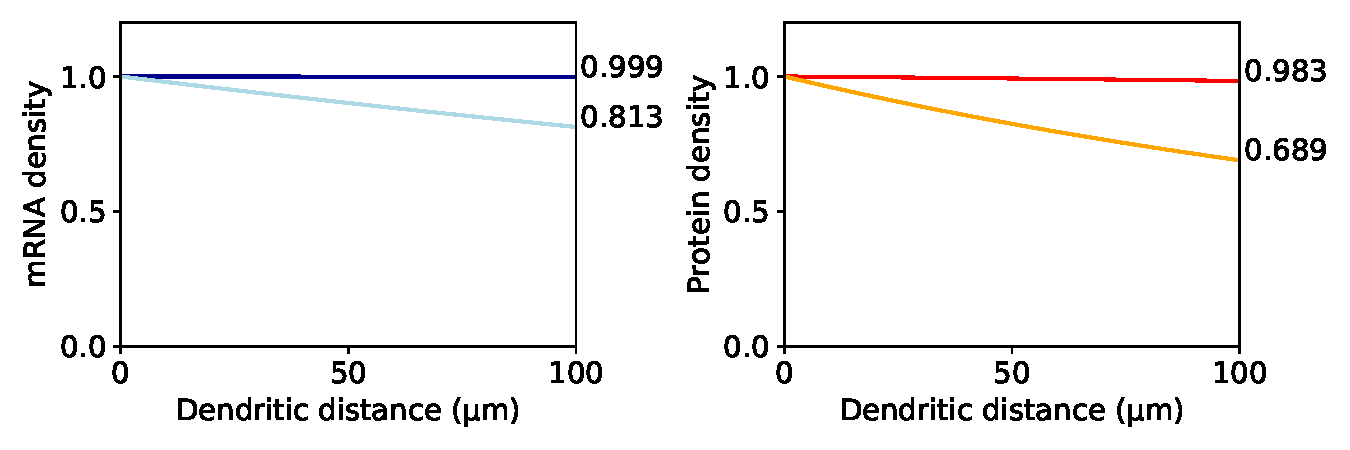
\includegraphics[width=\textwidth]{Figure1.pdf}
  \caption{Replication of the possible range of dendritic mRNA and protein distribution according to the literature.  Color code denotes the upper bound (dark blue and red) and lower bound (light blue and orange) for the respective distributions (\textbf{A}) mRNA distribution obtained for candidate values from the literature. Upper bound: $D_{R} = 0.0038\mu m^{2}/s$ and $\nu_{R}=1.3\mu m/s$. Lower bound:  $D_{R} = 0.003\mu m^{2}/s$ and $\nu_{R}=0.0058\mu m/s$. (\textbf{B}) Protein distribution obtained for candidate values from the literature.Upper bound: $D_{P} = 4.5\mu m^{2}/s$ and $\nu_{P}=0\mu m/s$. Lower bound:  $D_{P} = 0.023\mu m^{2}/s$ and $\nu_{R}=0\mu m/s$.} 
\end{figure}

In \textbf{Figure 2}, we show the influence of single parameter variations on mRNA and protein distribution. The initial parameters used are the one experimentally confirmed in the study: $D_{R}=3.4\cdot10^{-3} \mu m^{2}/s, \nu_{R}=6.7 \cdot 10^{-3} \mu m/s$. Qualitative inspection of the obtained graphs showed similar behavior and allowed to reach similar conclusions. 

\begin{figure}[H]
  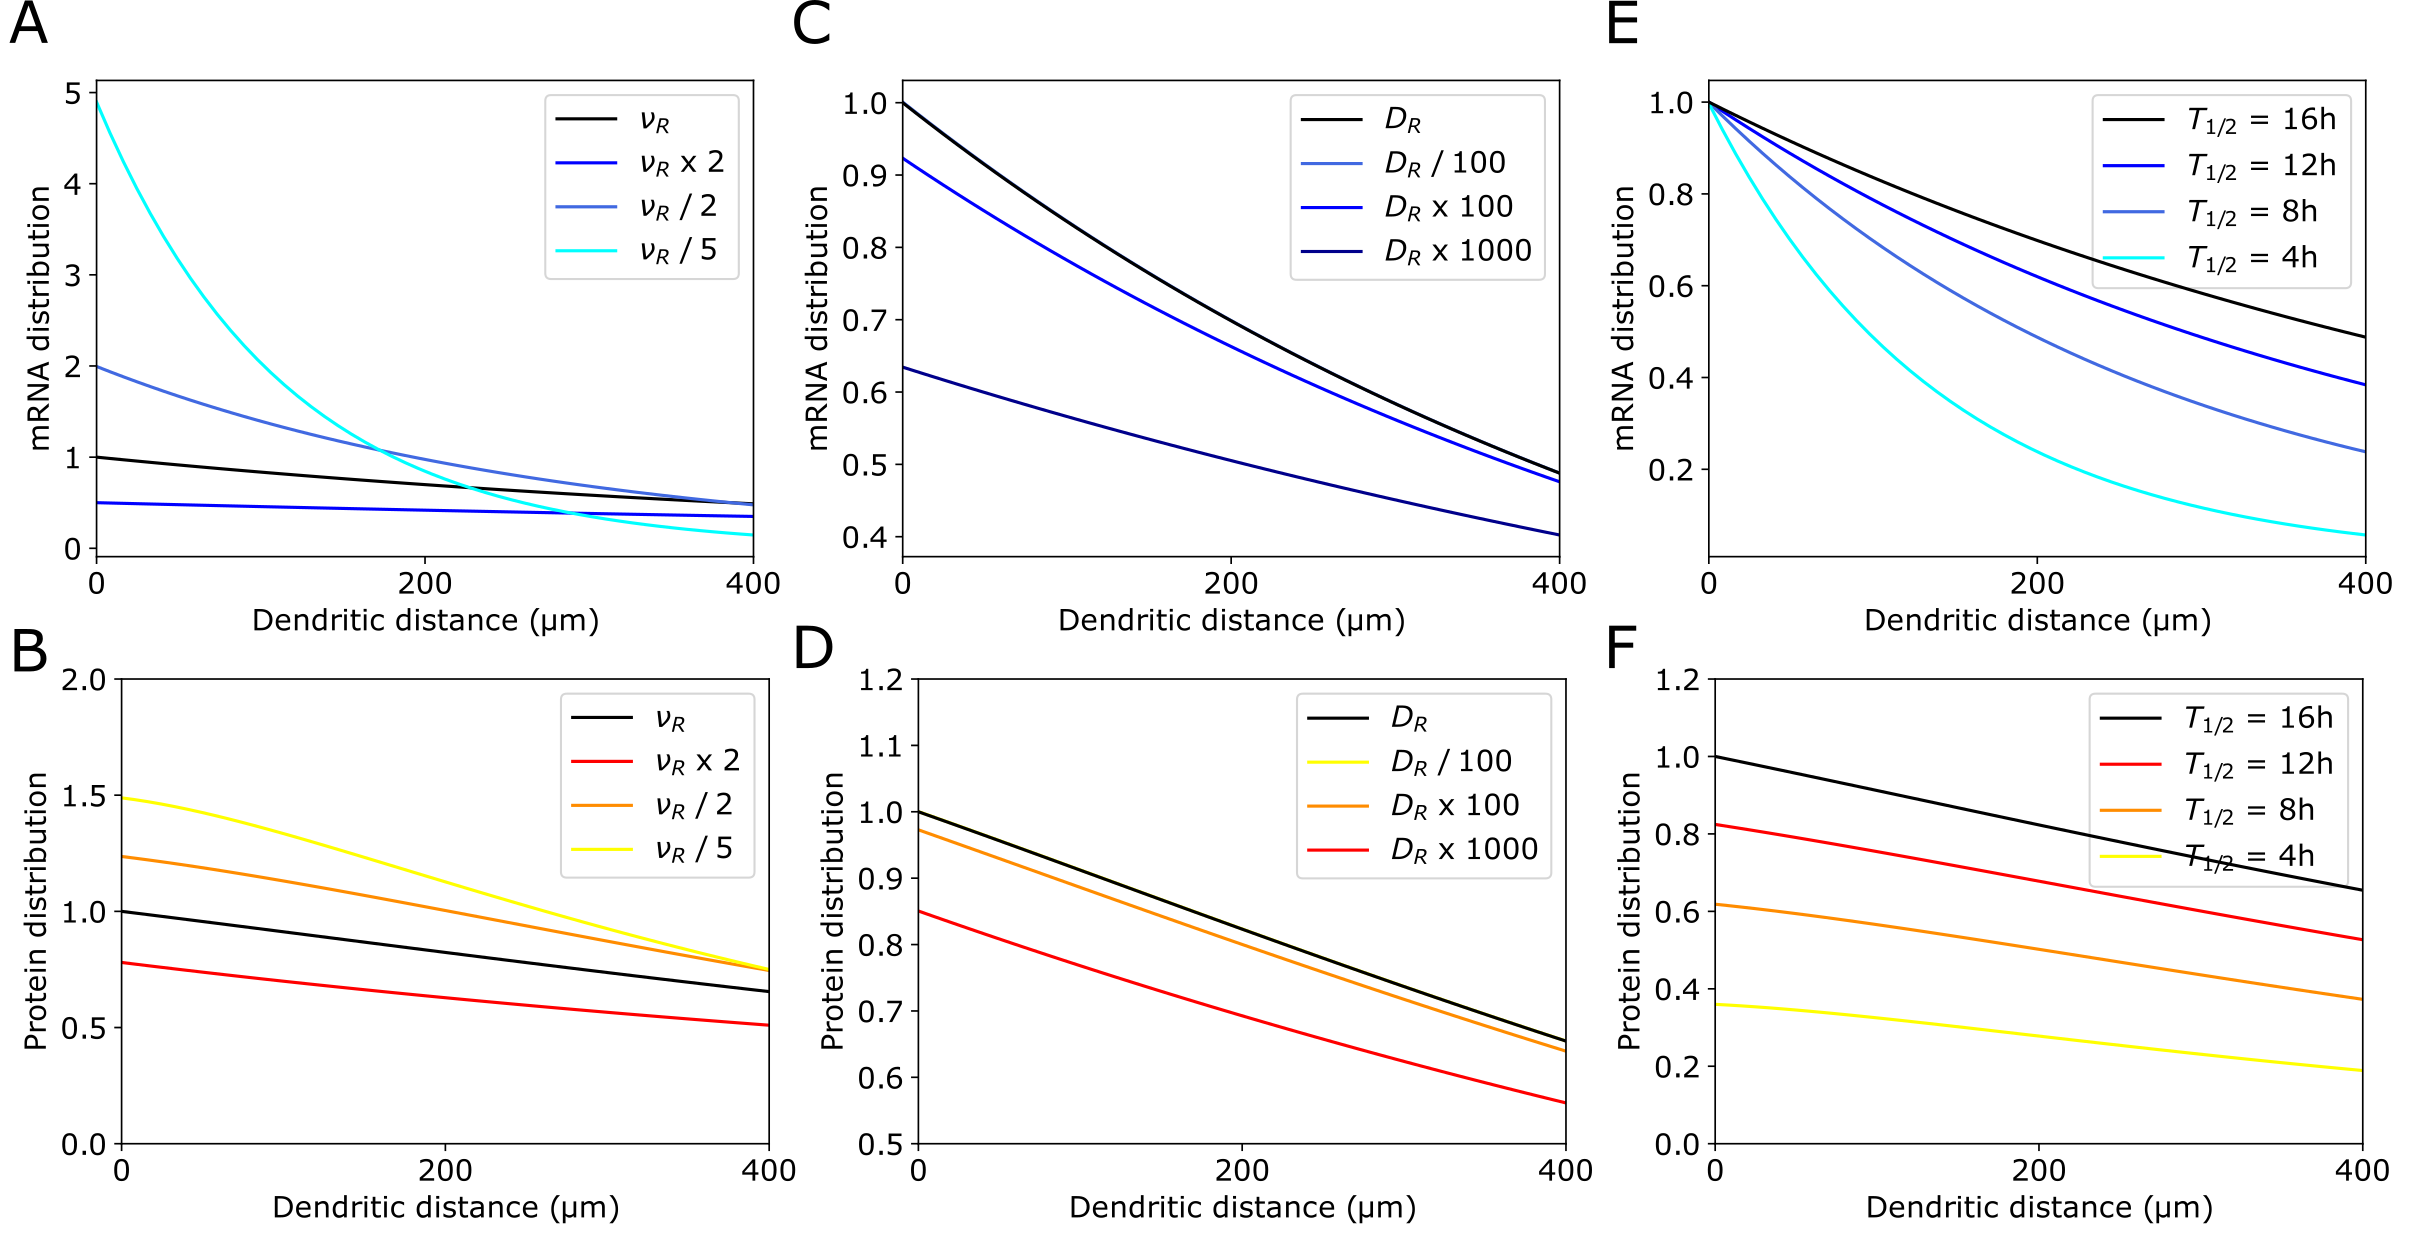
\includegraphics[width=\textwidth]{Figure2.png}
  \caption{Consequences of modulating mRNA parameters on mRNA and protein distributions. (\textbf{A, B}) Impact of mRNA velocity. (\textbf{D, E}) Impact of mRNA diffusion.(\textbf{F, G}) Impact of mRNA lifetime. In all panels, distributions were normalizxed to the original value. Alternative normalization were also explored and were successfully replicated (LINK ??)}
\end{figure}





